\documentclass[12pt,a4paper,openright,twoside]{book}
\usepackage[utf8]{inputenc}
\usepackage{algpseudocode}
\usepackage{algorithm}
\usepackage{disi-thesis}
\usepackage{code-lstlistings}
\usepackage{notes}
\usepackage{shortcuts}
\usepackage{acronym}

\school{\unibo}
\programme{Corso di Laurea Magistrale in Ingegneria e Scienze Informatiche}
\title{Fancy Title}
\author{Marco Raggini}
\date{\today}
\subject{Supervisor's course name}
\supervisor{Prof. Giovanni Ciatto}
\cosupervisor{Dott. Mattia Matteini}
\morecosupervisor{Dott. CoSupervisor 2}
\session{I}
\academicyear{2026-2027}

% Definition of acronyms
\acrodef{IoT}{Internet of Thing}
\acrodef{vm}[VM]{Virtual Machine}


\mainlinespacing{1.241} % line spacing in mainmatter, comment to default (1)

\begin{document}

\frontmatter\frontispiece

\begin{abstract}	
Max 2000 characters, strict.
\end{abstract}

\begin{dedication} % this is optional
Optional. Max a few lines.
\end{dedication}

%----------------------------------------------------------------------------------------
\tableofcontents   
\listoffigures     % (optional) comment if empty
\lstlistoflistings % (optional) comment if empty
%----------------------------------------------------------------------------------------

\mainmatter

%----------------------------------------------------------------------------------------
\chapter{Intro (motivazione, contesto, obiettivi)}
\label{chap:introduction}
%----------------------------------------------------------------------------------------

Write your intro here.
\sidenote{Add sidenotes in this way. They are named after the author of the thesis}

You can use acronyms that your defined previously,
such as \ac{IoT}.
%
If you use acronyms twice,
they will be written in full only once
(indeed, you can mention the \ac{IoT} now without it being fully explained).
%
In some cases, you may need a plural form of the acronym.
%
For instance,
that you are discussing \acp{vm},
you may need both \ac{vm} and \acp{vm}.

\paragraph{Structure of the Thesis}

\note{At the end, describe the structure of the paper}

\chapter{Background (tutto e solo ciò che serve a capire la tesi)}
I suggest referencing stuff as follows: \cref{fig:random-image} or \Cref{fig:random-image}

\begin{figure}
    \centering
    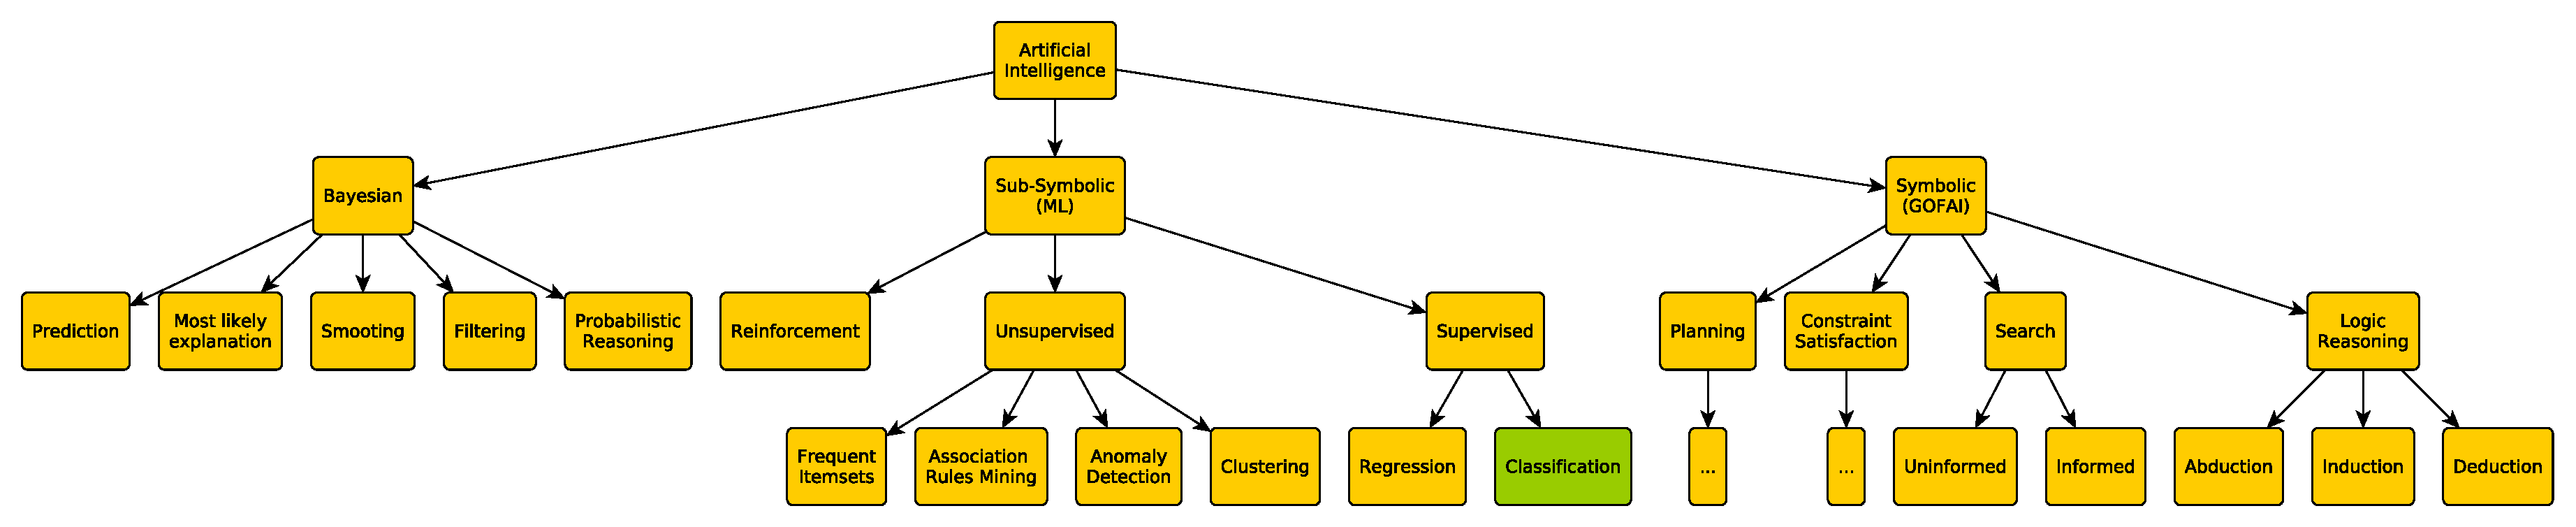
\includegraphics[width=.8\linewidth]{figures/random-image.pdf}
    \caption{Some random image}
    \label{fig:random-image}
\end{figure}

\section{LLM}
\section{LangChain \& LangGraph}
\section{Related Works (es. CoT, ToT, GoT)}

\chapter{Methodology / Design}
This chapter presents the proposed approach in detail.
We first formally define the problem and highlight the main challenges and requirements.
Then, we describe the proposed Graph of Thoughts, providing its formalization, including algorithmic details and execution strategies.
Lastly, we illustrate the approach with a concrete example to demonstrate its application.


\section{Problem statement}
\subsection{Task Definition}
Before introducing the proposed approach, we first formally define the problem addressed in this work.

Given an input problem $P$ expressed in natural language, the objective is to generate a solution $S$ together with a structured reasoning process $R$ that leads to $S$.
The reasoning representation $R$ is composed of multiple intermediate reasoning steps, which may form a non-linear structure. Each step represents a partial inference contributing to the final solution.
 The overall reasoning process should be coherent, interpretable, and effective in reaching correct answers.
\subsection{Challenges and Requirements}
LLMs are able to generate coherent text and perform reasoning, but as shown in the previous chapter, there are some limitations and challenges that need to be addressed:

\begin{itemize}
    \item \textbf{Limited explorations of alternatives}: The stardard approaches such as CoT and ToT, generates a single linear solution, which may not be sufficient to generate a good solution, especially for complex problems that may require more tries.
    \item \textbf{Black box reasoning}: The reasoning process of LLMs is often difficult to understand and interpret, the generated text is auto regressive and the model does not have a clear representation of the reasoning process, which makes it difficult to debug and improve the model.
    \item \textbf{Error propagation}: If there is an error in the early steps of the reasoning process, it will propagate to the solution. Without more exploration of alternatives, the model may not be able to recover from these errors and may produce incorrect solutions. 
\end{itemize}

In order to address these challenges, the requirements are formalized as follows:

\begin{itemize}
    \item \textbf{Exploration of alternatives}: If the LLM answer do not satisfy evaluation criterias, the model should be able to explore alternatives, which may require the ability to backtrack and try different reasoning paths. 
    \item \textbf{Separation of reasoning}: The system should allow starting a new reasoning process independently if a path leads to an incorrect solution, without affecting other trajectories.
    \item \textbf{Structured and interpretable reasoning}: The reasoning process should be captured in a structured representation that enables traceability, interpretability, and evaluation of intermediate steps.
\end{itemize}

\section{The proposed approach}
\subsection{Overview of the approach}
The approach proposed in this thesis is based on the Graph of Thoughts paradigm. 
In this framework, the reasoning process is modeled as a dynamic graph, where nodes represent intermediate thoughts and the Large Language Model (LLM) guides both the expansion of the graph and the decision of when to terminate the reasoning process.

Given an input problem ($P$), the system incrementally constructs a graph according to a set of high-level rules. 
These rules are designed to balance the exploration of multiple reasoning paths with the need for coherent and effective problem solving. Additionally, they encourage the use of external tools, which plays a key role in improving traceability and interpretability of the reasoning process.
At a high level, the approach can be described through the following phases:
\begin{enumerate}
\item \textbf{Initialization:} the input problem ($P$) is used to create the root node of the graph.
\item \textbf{Graph expansion:} the system generates multiple nodes corresponding to different candidate reasoning paths.
\item \textbf{Reasoning:} each path is progressively expanded by producing intermediate thoughts ($R$), until a candidate solution is reached.
\item \textbf{Evaluation and refinement:} the generated solutions are evaluated, and the system may revise previous steps, explore alternative paths, or leverage external tools to improve the reasoning process.
\item \textbf{Backtracking:} if a path leads to an unsatisfactory solution, the system can backtrack to previous nodes and explore alternative paths, giving also feedbacks for improving the reasoning process.
\item \textbf{Crafting:} if the system identifies the need for a new tool to solve the problem, it can craft a new tool and use it in the reasoning process.
\item \textbf{Divide Thought:} if the LLM has difficulties in solving the problem, it can decide to divide the problem into two subproblems.
\item \textbf{Termination:} the process continues until a satisfactory solution is found or a predefined stopping condition is met ($S$).
\end{enumerate}

Some of the phases described above are sequential (e.g. Initialization $\rightarrow$ Graph expansion $\rightarrow$ Reasoning $\rightarrow$ Evaluation and refinement), while others can be explored in a more flexible way (e.g. Backtracking, Crafting, Divide Thought and Termination can be triggered during the evaluation phase).

\subsection{Motivation for using GoT}
The GoT paradigm is chosen for the potential that this structure offers in terms of exploration, combination of different resoning paths and the ability to backtrack in order to recover from errors.
\\
The second motivation about the use of GoT, as mentioned in the previous chapter, is the fact that the GoT research is still in its early stages, so its potential is not yet fully explored.

\section{Formalizations}
Now that we have described the proposed approach at a high level, we can provide a more formal description of what the system does, starting from the input and the expected output.

\subsection{Assumptions}
In order to simplify the problem and focus on the core aspects of the GoT paradigm, we make the following assumptions:

\begin{itemize}
    \item \textbf{LLM capabilities}: We assume that the LLM has enought capabilities to use external tools, to craft tool if needed, to evaluate the generated solutions and to generate intermediate thoughts that are coherent and relevant to the problem at hand. This assumption is strictly dependent on the size of the LLM that we are using.
    \item \textbf{Tool-Centric Problem Domain}: We assume the input problems belong to a class of tasks that cannot be solved through direct, zero-shot text generation alone. The problems are assumed to require non-trivial reasoning sequences and at least one interaction with an external environment or tool (e.g., a calculator, a search engine, or a code interpreter).    \
    \item \textbf{Thought Atomicity}: We assume that each node in the graph represents an "atomic" step of reasoning or a single functional operation. While the internal process of the LLM remains a black box, the output of each node is treated as a discrete state in the problem-solving space.
    \item \textbf{Resource Finiteness}: We assume the existence of an upper bound on the graph depth and the number of LLM invocations to ensure the termination of the process and to mitigate potential infinite loops caused by recursive backtracking. This assumptions is also valid for time and computational resources, which are limited and should be taken into account when designing the system.
\end{itemize}

\subsection{Graph of Thoughts Formalization}
Before describing the graph algorithm in details, we need to formalize some aspects of the graph structure, in particular, the difference between static and dynamic graph.
\subsubsection{Static Graph Structure}
As \textbf{static graph}, we refer to the graph structure that is defined at the beginning of the process, which includes the definition of nodes and edges, as well as the rules for how they can be connected. The static graph structure provides a framework for how the reasoning process can be represented and how different thoughts can be connected to each other.
This structure can't be changed during the process and it represents the "rules" of the graph.
\\\\
The static graph structure is defined as $G_s = (S, T)$, where $S$ is the set of possible logical states (e.g. Evaluation, Backtracking, Crafting etc.) and $T$ is the set of possible transitions between these states. 
The states are defined and they are the following:

\begin{itemize}
    \item \textbf{\_\_start\_\_ and \_\_end\_\_}: the start and end states of the process. The \texttt{\_\_start\_\_} is the first state reached and the \texttt{\_\_end\_\_} is the last reached in the process. These represent entry and exit points and are visited exactly once per execution.
    \item \textbf{goal}: this is the first real state. The system starts with the user prompt and the \texttt{goal} represents the problem to answer. From here, the system starts to generate thought paths that can be explored in order to solve the problem.
    \item \textbf{tool\_reasoning}: this is the starting point of a reasoning path. From here the system starts to think about how to solve the problem without solving it directly in order to force the reasoning to the LLM. The main focus of this state is about how to use the tools or, in some cases, how to craft them.
    \item \textbf{tool\_calling}: this state is reached after the \texttt{tool\_reasoning} and it represents the moment in which the system should call the tool or just generate the solution if the tool is not needed.
    \item \textbf{response\_evaluation}: is reached after the \texttt{tool\_calling} or the \texttt{reasoning\_mode} and it represents the moment in which the system evaluates the generated response of the reasoning process. This moment is crucial in this structure because the evaluation decides what state must be reached next.  
    \item \textbf{backtrack}: is reached when an evaluation doesn't satisfy the LLM criteria for become a solution. This state allows to backtrack to a previous not visited reasoning path and explore it, giving also feedbacks to the LLM about what is wrong with the previous path.
    \item \textbf{crafting}: is reached when, after an evaluation, the system identifies that a new tool is needed to solve the problem. In this state, the LLM try to craft a tool that permits to solve or help to solve the problem and then a new reasoning path is chosen for exploration.
    \item \textbf{reasoning\_mode}: is a different approach to solve the problem. If the \texttt{tool\_reasoning} and \texttt{tool\_calling} states are focused on how to use the tools, the \texttt{reasoning\_mode} is focused on how to solve the problem using divide-et-impera system, so it is more focused on the reasoning capabilities of the LLM. This state is used when the system has difficulties in solving the problem.
    \item \textbf{chat\_completion}: acts as a fallback mechanism to ensure a response is provided even when complex reasoning paths fail. This state is reached when the system has explored all the possible paths and it is not able to find a solution, so it just call the LLM to generate a solution without any constraint, in order to guarantee the termination of the process.
\end{itemize}

We partition the set of transitions $T$ into two disjoint subsets: $T = T_d \cup T_c$ where:
\begin{itemize}
    \item $T_d$ is the set of deterministic transitions, where the next state is uniquely determined by the completion of the current state’s task.
    \item $T_c$ is the set of conditional transitions, where the next state is determined by a selection function $f: \text{output} \to S$, typically driven by the LLM's internal evaluation or a logic-based heuristic.
\end{itemize}

The static graph structure defines the possible paths that can be taken during the reasoning process, but it does not define which path will be taken in a specific execution.

\begin{figure}
    \centering
    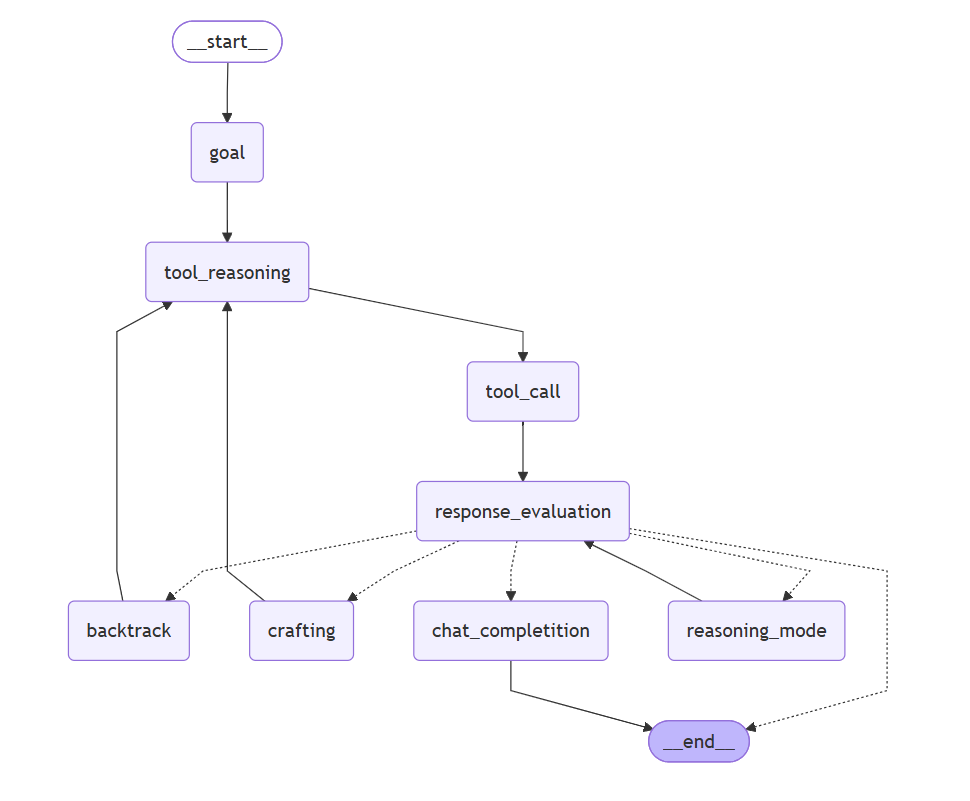
\includegraphics[width=.8\linewidth]{figures/static_graph.png}
    \caption{Static Graph Structure: continuous lines represent direct transitions, while dashed ones represent conditional transitions.}
    \label{fig:static-graph}
\end{figure}

\subsubsection{Dynamic Graph Semantics}
We represent the system as a directed graph $G = (N, E)$, where:
\begin{itemize}
    \item $N$ = $\{n_1, n_2, ..., n_m\}$ is the set of nodes, where each node $n_i$ is a 5-tuple: $n_i = (s_i, a_i, p_i, r_i, m_i)$, where $s_i$ is the state that the node represents, $a_i$ is the agent that executes the node, $p_i$ is the prompt sent to the LLM to generate the thought, $r_i$ is the reasoning process generated by the LLM in response to the prompt, and $m_i$ represent the metadata associated with the node, in particular the tool used during the thought generation.
    \item $E$ = $\{e_1, e_2, ..., e_k\}$ is the set of directed edges, where each edge $e_j = (n_{i1}, n_{i2}, h_j) \in E$ represents a transition from node $n_{i1}$ to node $n_{i2}$ with the message history $h_j$. The message history $h_j$ is a sequence of interactions happened in the nodes before. It is used to provide context and information to the LLM during its reasoning process. The message history sometimes is manipulated by the system in order to provide the right behaviour to the LLM (e.g. crafting a tool instead of using it).
\end{itemize}

\subsubsection{Agents Definition}
In the proposed system, we define multiple agents in order to manage different states of the graph and to provide a more customized behaviour for each state.
Matematically we define an agent $a \in A$ as a function: 
\begin{equation}
    a: (h_j, p_i) \to (r_i, m_i)
\end{equation}
In particular, we define the following agents:
\begin{itemize}
    \item \textbf{Starting agent}: It is an expert of tool usage, but his role is to reason about how to solve the problem with the tools, if there is a need of a new tool or if the problem does not require them.  
    \item \textbf{Tool agent}: It is also an expert of tool usage. Its role is to follow the instructions of the starting agent and provide a solution by using the tools.
    \item \textbf{Judge agent}: It is an expert of evaluation. This agent is crucial for the system because it is responsible for judge the generated solution and decide it can be the final answer or it needs to be revised. This agent is also responsible for decide if a new tool is needed. 
    \item \textbf{Crafter agent}: It is an expert of tool crafting. It is used for crafting a new tool.
    \item \textbf{Reasoning agent}: It is an expert of reasoning. Its role is to analyze the problem and generate potential solutions using the divide-et-impera approach.
    \item \textbf{Chat completition agent}: It is a generalist agent, it is used as a fallback mechanism to generate a solution without any constraint when the system has explored all the possible paths and it is not able to find a solution.
\end{itemize}

\subsection{Algorithm}

\subsubsection{High-level Description}
The algorithm follows the static graph's structure and in every state, it creates a new node of the dynamic graph.
\\\\
As we say previously, the system follows a set of rules (static graph) and its logical process is:
\begin{enumerate}
    \item Starting point: The user sends a prompt to the system that creates the \texttt{goal} node and four different reasoning paths composed by three \texttt{tool\_reasoning} nodes and one \texttt{reasoning\_mode} node. The number of tool reasoning paths created is arbitrary, it is chosen by observing the system's behaviours during its runs. A higher number of reasoning paths can lead to more solutions, but the cost in terms of time and tokens increases.
    \item Tool reasoning: The system expand a \texttt{tool\_reasoning} node previously created and calls the LLM into it. The response is memorized in the message history and a new \texttt{tool\_call} node is created using the message hisotry as context.
    \item Tool call: In this state, the LLM is expected to resolve the problem by leveraging the context provided by the preceding node. Since LLMs are stochastic auto-regressive models, we cannot deterministically predict the exact output; however, the system is designed to enforce instruction-following through the provided context. The expected behavior is for the model to generate a response that incorporates tool calls (if deemed necessary) or a direct solution, effectively bridging the gap between reasoning and action. The \texttt{response\_evaluation} node is created for the next step.
    \item Evaluation: The LLM-as-a-judge method is used to evaluate the response. The evaluation is based by the format of the response (sometimes the response should have a fixed format), the correctness of the result and the explanation of the process. The judge agent has the entire message history, so it has a fully vision of the reasoning process. In order to evaluate the response, the LLM must score the solution to a number between 0 and 5, where 5 is the maximumn, and also give it a score to the problem complexity. These two parameters are used to decide if the response can pass or not. 
    The evaluation threshold is dynamically adjusted based on the problem complexity:
    \begin{equation}
    S \geq 5.5 - 0.5 \cdot C
    \end{equation}
    Where $S$ is the score and $C \in [1,...,5]$ is the complexity. If the problem is too complex, a non-perfect response may be accepted. The logic behind it is that if the LLM has difficulty to find a solution, the logical soundness of the reasoning process is prioritized over the absolute precision of the final output.  
    The LLM can also understand, usually hinted by the tool call response, that a new tool is needed. In this case the next node will be \texttt{crafting}. 
    \begin{enumerate}
        \item Backtrack: If the response does not pass the evaluation and there at least one \texttt{tool\_reasoning} node not expanded, the system backtracks in order to explore and expand another reasoning path. In this phase, the message history is manipulated, the system retainsonly the feedback the judge agent generates to improve the reasoning process.     
        \item Crafting: If the judge agent identifies that the available tools are insufficient, it triggers a \texttt{crafting} state, provided there is at least one reasoning path available for exploration. In this state, a specialized crafter agent generates a new tool definition. This process uses the original problem context ($P$) and the judge's feedback as a specification. Once the tool is crafted, the system resumes the exploration by expanding a new reasoning path that can now leverage the newly created capability.
        \item Reasoning: When the response does not pass the evaluation and there is no \texttt{tool\_reasoning} node available, the system explores the last path. In this case, the reasoning path is a different reasoning approach. It has the possibility to divide the thought into two parallel sub-tasks in order to divide the complexity of the single prompt. The two prompt should be indipendent of each other. 
    \end{enumerate}
    \item Chat completition: Once all reasoning paths have been explored and have failed to yield a correct solution, the last solution is the standard LLM response.
\end{enumerate}

\newpage
\subsubsection{Pseudocode}
For a complete comprehention of the crucial steps of the system, some snippets of pseudocode are presented here.
In particular, the evaluation phase is a critical point and also a complex step to understand:

\begin{algorithm}
\begin{algorithmic}[1]
\Procedure{evaluate}{message\_history}
    \State $evaluation \gets$ judge\_agent.call("Evaluate this solution", message\_history)
    \State $nodes\_avail \gets$ exist\_node\_tool\_available()
    \State $threshold \gets$ COMPLEXITY\_THRESHOLD $-$ COMPLEXITY\_COEFFICIENT $\cdot$ problem\_complexity

    \If{$evaluation.score \geq threshold$}
        \State \Return \_\_end\_\_

    \ElsIf{$evaluation.score < threshold$ \textbf{and} $nodes\_avail$ \textbf{and} evaluation.need\_tool\_crafting}
        \State \Return ``crafting''

    \ElsIf{$evaluation.score < threshold$ \textbf{and} $nodes\_avail$}
        \State \Return ``backtrack''

    \ElsIf{$evaluation.score < threshold$ \textbf{and} $!nodes\_avail$ \textbf{and} exist\_reasoning\_node\_available()}
        \State \Return ``reasoning\_mode''

    \Else
        \State \Return ``chat\_completition''
    \EndIf
\EndProcedure
\end{algorithmic}
\end{algorithm}

\subsection{Illustrative Example}
\subsubsection{Example Task}
\subsubsection{Step-by-step Execution}

\chapter{Implementation}
\section{Dettagli da ingegnere del software}
\subsection{Git workflow}
\subsection{Graph implementation}
\subsection{Crafting methodology}
\section{Tools, libraries, framework used}
\subsection{Poetry}
In order to create a virtual and reproducible environment, the project uses Poetry as dependency resolver.
\subsection{LangChain/LangGraph}
As mentioned in the previous chapter, LangChain is a framework that facilitates the integration with LLMs and the management of the reasoning process.
\\
In this project, LangChain is used in the following steps:
\begin{itemize}
    \item \textbf{LLM/agent calls}: LangChain provides classes and methods to call third part LLMs and to create agents with specific behaviours.  
    \item \textbf{Tools management}: It offers a simple way to create and assign tools to the agents.
    \item \textbf{Graph management}: LangGraph permits to create and manage the static graph structure.
    \item \textbf{Message history management}: LangChain provides a sets of classes that permit to save and manipulate the message history in order to provide a different context to the different agents and to implement the backtracking mechanism. It is also used to classify the message in different categories: \textbf{System}, \textbf{AI} and \textbf{User} messages, which was useful for a better customization of the prompts.
    \item \textbf{Call limits}: LangChain provides mechanisms to limit the number of calls to the LLMs, which is useful to control the cost and performance of the system. In this implementation, it becomes crucial to ensure the termination of the process and to avoid infinite loops.
\end{itemize}

\subsection{Gemini Framework}
The Gemini framework is used to call the Gemini LLMs, which are the LLMs used in this project. In particular, the Gemini APIs offer the possibility to customize the format of the agent response.
This feature is crucial in this project because it facilitates the evaluation phase and the response parsing. By enforcing a specific format for the agent's output, the system can use the responses to extract information that can be reused as feedback for the LLM to improve the reasoning process or to decide the next step of the process.
\subsection{MLflow}
MLflow is an open-source platform for managing the machine learning lifecycle, including experimentation, reproducibility and deployment. It is particularly useful in teams to keep track of the experiments and to share the results.
\\\\
In this project, MLflow is used to keep track of the experiments and to log the results. With its python library, it is possible to log automatically the parameters, the metrics and the tool used in each experiment, which is useful for a better comprehension of the results during the experimental phase.
\\\\
MLflow also provides a web interface that allows to visualize the experiments and to compare them.
It also provides a bunch of metrics that are used in the evaluation phase, such as the number of tools used, the token usage and its average, the number of error and the latency of each call.  
\subsection{Mermaid}

\section{System Architecture}
\subsection{System folders}

\chapter{Experiments}
\section{Descrizione setup sperimentale (quali classi di benchmark, cosa testi per ogni benchmark, come lo misuri)}
\section{Per ogni classse di benchmark:}
\subsection{Descrizione della classe di benchmark}
\subsection{Risultati quantitativi (metriche, grafici, tabelle)}
\subsection{Analisi qualitativa (esempi di output, errori comuni, casi di successo)}

\chapter{Discussion}
\section{Interpretazione dei risultati (funziona bene in questi casi, funziona male in questi altri, suppongo sia perchè...)}
\section{Confronto con altri approcci (es. CoT, ToT)}
\subsection{Se ho tempo riprodurre i test di altri esperimenti}
\subsection{Altrimenti comparazione a parole}
\section{Limiti del mio approccio (es. non funziona bene in questi casi, perchè...)}

\chapter{Conclusion}
\section{Recap degli obiettivi e ricapitolo di come sono stati raggiunti}
\section{Implicazioni future}

%----------------------------------------------------------------------------------------
% BIBLIOGRAPHY
%----------------------------------------------------------------------------------------

\backmatter

\nocite{*} % Remove this as soon as you have the first citation

\bibliographystyle{alpha}
\bibliography{bibliography}

\begin{acknowledgements} % this is optional
Optional. Max 1 page.
\end{acknowledgements}

\end{document}
